\documentclass[11pt,a4paper]{article}

\usepackage[american]{babel}
\usepackage[T1]{fontenc}
\usepackage[utf8]{inputenc}
\usepackage{lmodern}
\usepackage{microtype}
\usepackage[a4paper,margin=22mm,headheight=14pt]{geometry}
\usepackage{graphicx}
\usepackage{booktabs}
\usepackage{tabularx}
\usepackage{enumitem}
\usepackage{xcolor}
\usepackage{fancyhdr}
\usepackage{hyperref}
\usepackage{tikz}
\usepackage[most]{tcolorbox}
\usepackage[section]{placeins}
\usepackage{libertine}
\usetikzlibrary{arrows.meta,positioning,fit}

\definecolor{avacblue}{HTML}{1F5C99}
\definecolor{avaclight}{HTML}{EAF3FA}
\definecolor{avacgray}{HTML}{4E5963}
\definecolor{waveblue}{HTML}{2C7FB8}
\definecolor{wavefill}{HTML}{E5F5F9}
\definecolor{warnfill}{HTML}{FFF4D6}
\definecolor{warmred}{HTML}{C0392B}

\hypersetup{
  colorlinks=true,
  linkcolor=avacblue,
  urlcolor=avacblue,
  pdftitle={AVAC4QGIS Tutorial},
  pdfauthor={LHE--EPFL},
  pdfsubject={Tutorial for AVAC4QGIS 0.5.14}
}
\setlist[itemize]{leftmargin=*,itemsep=3pt,topsep=4pt}
\setlist[enumerate]{leftmargin=*,itemsep=5pt,topsep=4pt}
\setlength{\parindent}{0pt}
\setlength{\parskip}{5pt}
\renewcommand{\arraystretch}{1.15}

\pagestyle{fancy}
\fancyhf{}
\fancyhead[L]{\small AVAC4QGIS Tutorial}
\fancyhead[R]{\small Version 0.5.14}
\fancyfoot[C]{\thepage}

\newcommand{\control}[1]{\textbf{#1}}
\newcommand{\pathcode}[1]{\texttt{#1}}
\newcommand{\uiscreenshot}[2]{%
  \begin{figure}[htbp]
    \centering
    \includegraphics[width=.88\textwidth,height=.52\textheight,keepaspectratio]{images/#1}
    \caption{#2}
  \end{figure}
}
\newcommand{\resultfigure}[2]{%
  \begin{figure}[htbp]
    \centering
    \includegraphics[width=.86\textwidth,height=.50\textheight,keepaspectratio]{images/#1}
    \caption{#2}
  \end{figure}
}
\newenvironment{notebox}{%
  \begin{tcolorbox}[colback=avaclight,colframe=avacblue,boxrule=.6pt,
                     arc=2pt,left=6pt,right=6pt,top=5pt,bottom=5pt]
  \small
}{%
  \end{tcolorbox}
}
\newenvironment{importantbox}{%
  \begin{tcolorbox}[colback=warnfill,colframe=warmred,boxrule=.6pt,
                     arc=2pt,left=6pt,right=6pt,top=5pt,bottom=5pt]
  \small
}{%
  \end{tcolorbox}
}

\title{\textbf{AVAC4QGIS Tutorial}\\[6pt]
       \large From an avalanche release to an optional lake impulse wave}
\author{LHE--EPFL, Switzerland}
\date{August 28, 2026}

\begin{document}
\maketitle
\thispagestyle{empty}

\begin{notebox}
This tutorial follows the interface distributed with AVAC4QGIS 0.5.14. It
uses the public demonstration terrain and avalanche-release layer supplied in
the repository. The values visible in screenshots belong to one demonstration
workspace; they are not recommended values for another site. Choose scientific
parameters from the data and objectives of the case being studied.
\end{notebox}

\vfill
\begin{center}
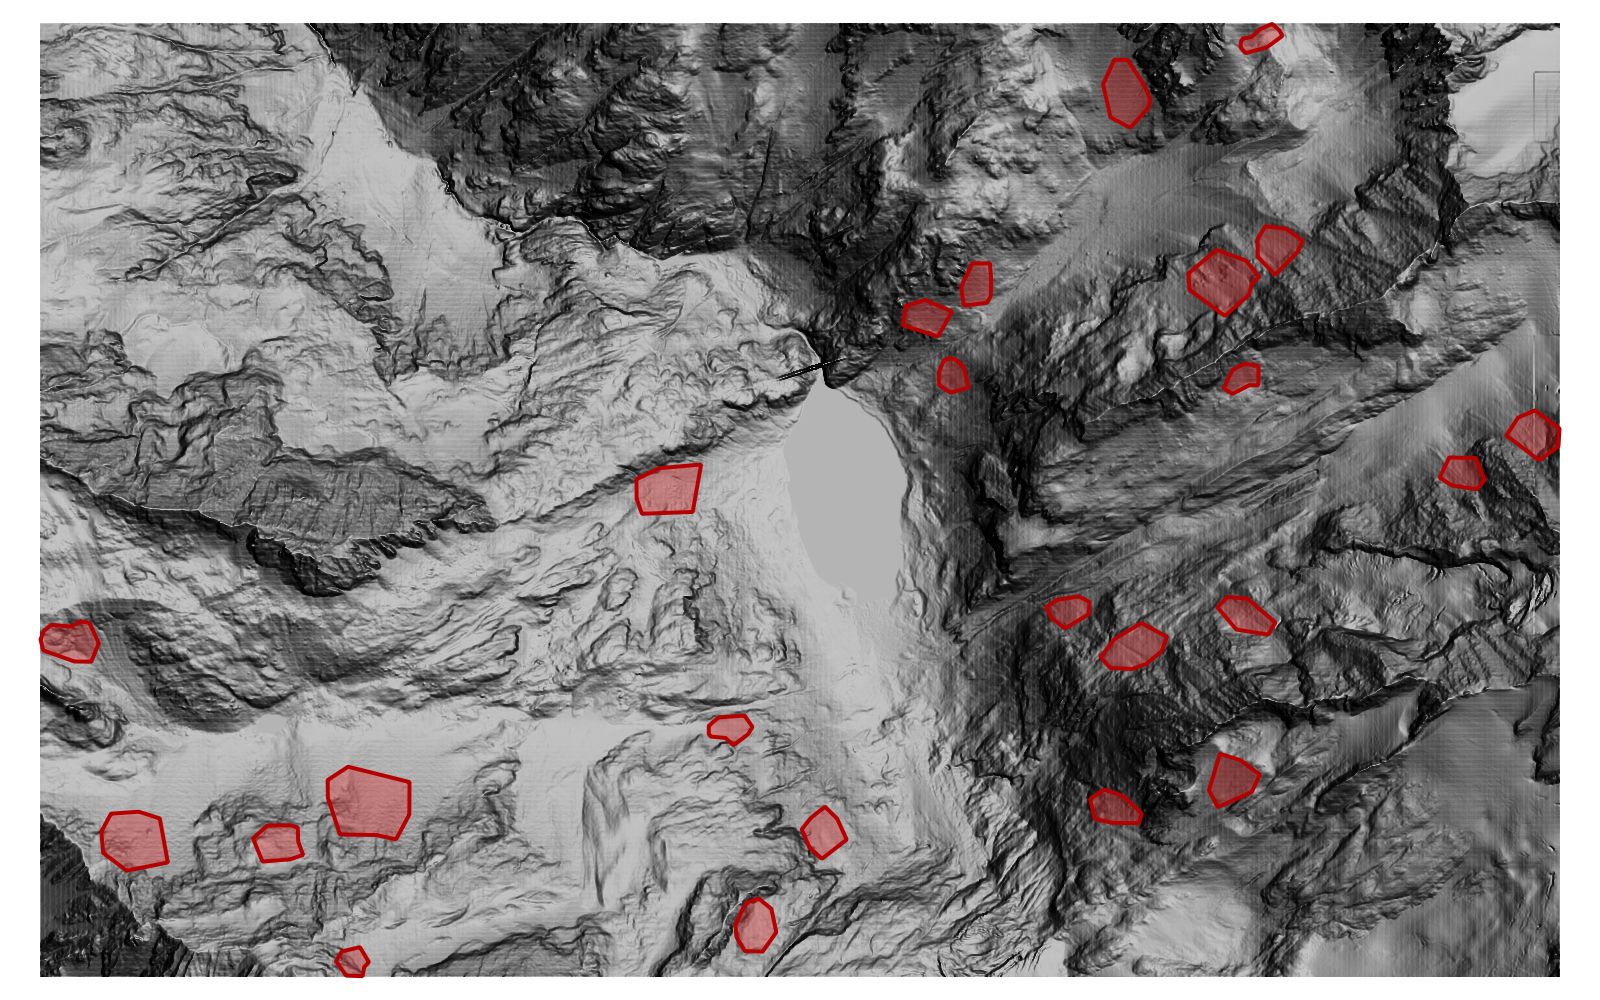
\includegraphics[width=.92\textwidth,height=.48\textheight,keepaspectratio]{images/tutorial_input_layers.png}

\small The tutorial terrain DEM displayed as hillshade, with the release polygons in red.
\end{center}
\vfill

\clearpage
\tableofcontents
\clearpage

\part{General workflow}

\section{What AVAC4QGIS simulates}

AVAC4QGIS brings two separate depth-averaged solvers into one QGIS workflow:

\begin{itemize}
  \item \control{AVAC} simulates the release, acceleration, propagation, and
        deposition of an avalanche over a terrain DEM.
  \item \control{WAVE} simulates the water response in a lake or reservoir.
        It is optional and is enabled only when the avalanche-to-water
        interaction is part of the case.
\end{itemize}

An AVAC-only study ends after the avalanche results are produced. In a coupled
study, WAVE starts from a completed AVAC run and converts the avalanche flux
entering the lake through the shoreline into internal water mass and momentum
sources. WAVE then propagates the resulting impulse wave. Enabling WAVE does
not change or rerun AVAC.

\section{Tutorial data and preparation}

Load the following two solver inputs from the repository's
\pathcode{tutorial/} directory into the QGIS project:

\begin{center}
\begin{tabularx}{\textwidth}{@{}lX@{}}
\toprule
File & Purpose \\
\midrule
\pathcode{topo\_cut\_dam\_1m.tif} & Terrain elevation raster used by AVAC and, in the coupled example, by WAVE. \\
\pathcode{avalanches.geojson} & Polygon layer defining the possible avalanche releases. \\
\bottomrule
\end{tabularx}
\end{center}

The optional georeferenced image \pathcode{satellite.png}, together with its
\pathcode{satellite.pgw} world file, is only a visual background. It is not a
solver input.

\resultfigure{tutorial_input_layers.png}{The two required tutorial layers: the DEM displayed with a hillshade renderer and the release-polygon layer.}

\section{The persistent controls above the tabs}

Open the plugin from \control{Plugins $>$ AVAC4QGIS}. The controls above the
tabs apply to the complete plugin workflow:

\begin{enumerate}
  \item Set the \control{AVAC Working Directory} to a writable case folder.
        Prepared runs, result rasters, previews, and exports are stored there.
  \item Leave \control{Enable Lake-Wave Extension} off for an avalanche-only
        case. Turn it on to show the WAVE Parameters and WAVE Run tabs.
  \item \control{Save Case} records the complete plugin setup, including the
        working directory, persistent input-layer paths, visible AVAC settings,
        and WAVE settings when the extension is enabled.
  \item \control{Load Case} restores that complete setup after QGIS or the
        plugin has been closed.
\end{enumerate}

\begin{notebox}
\control{Load Case}/\control{Save Case} concern the complete plugin. The
configuration buttons at the bottom of AVAC Parameters and WAVE Parameters
concern only the corresponding solver settings. A QGIS memory layer must be
saved to disk before it can be restored portably from a case file.
\end{notebox}

\uiscreenshot{tutorial_overview.png}{The complete AVAC4QGIS dock. Persistent case controls remain above every workflow tab.}

\clearpage
\part{AVAC: preparing and running the avalanche}

\section{Minimum inputs and AVAC configuration files}

Only two map inputs are required for a new AVAC simulation: a terrain DEM and
a release polygon. The four accordions in AVAC Parameters collect those inputs
and the release, rheology, and numerical settings.

At the bottom of the tab, \control{Load Configuration} reads AVAC settings
from an AVAC YAML file and \control{Save Configuration} writes the current
AVAC settings. These buttons are useful for transferring the avalanche model
setup without replacing the rest of a saved plugin case. Load a configuration
before reviewing the four accordions, because loaded values replace their
current contents.

\section{AVAC Inputs accordion}

\begin{enumerate}
  \item Select \control{Tutorial terrain DEM} as the \control{DEM raster
        layer}.
  \item Select \control{Tutorial avalanche release polygons} as the
        \control{Release polygon layer}.
  \item If the layer contains several features, select the releases to be
        simulated in the QGIS map. If no feature is selected, all usable
        release features are used.
\end{enumerate}

\begin{importantbox}
The DEM must have a valid projected CRS, finite usable cells, and square
pixels. The release layer must be a valid polygon or multipolygon layer with a
valid CRS. At least one selected release must overlap a usable DEM cell. AVAC
uses the full usable DEM extent.
\end{importantbox}

\uiscreenshot{tutorial_avac_inputs.png}{AVAC Inputs accordion with the tutorial DEM and release layer selected.}

\section{Release / initial conditions accordion}

This page converts release polygons into the initial mobile avalanche depth.
Choose the release-depth interpretation, the reference terrain or slope
quantity used by that interpretation, and any volume or depth scaling required
by the selected method. The initial AVAC depth is zero outside the release
polygons: the model does not silently add a stationary snow cover.

Use \control{Preview Initial Depth} before preparation. The preview writes a
raster in the working directory and loads it in QGIS, allowing the selected
release features, rasterization, and resulting initial volume to be checked.

\begin{notebox}
The release layer represents the initial moving volume. Its polygons must not
be confused with a computational mask or with the later lake polygon.
\end{notebox}

\uiscreenshot{tutorial_avac_release.png}{Release / initial conditions accordion. Review the method, its inputs, and the preview control.}

Figure~\ref{fig:initial-depth-preview} shows the spatial check produced for
the tutorial's uniform-depth release. Colored cells are the initial mobile
depth that AVAC will place inside the selected polygons; the transparent
background confirms that no depth was created elsewhere.

\begin{figure}[htbp]
\centering
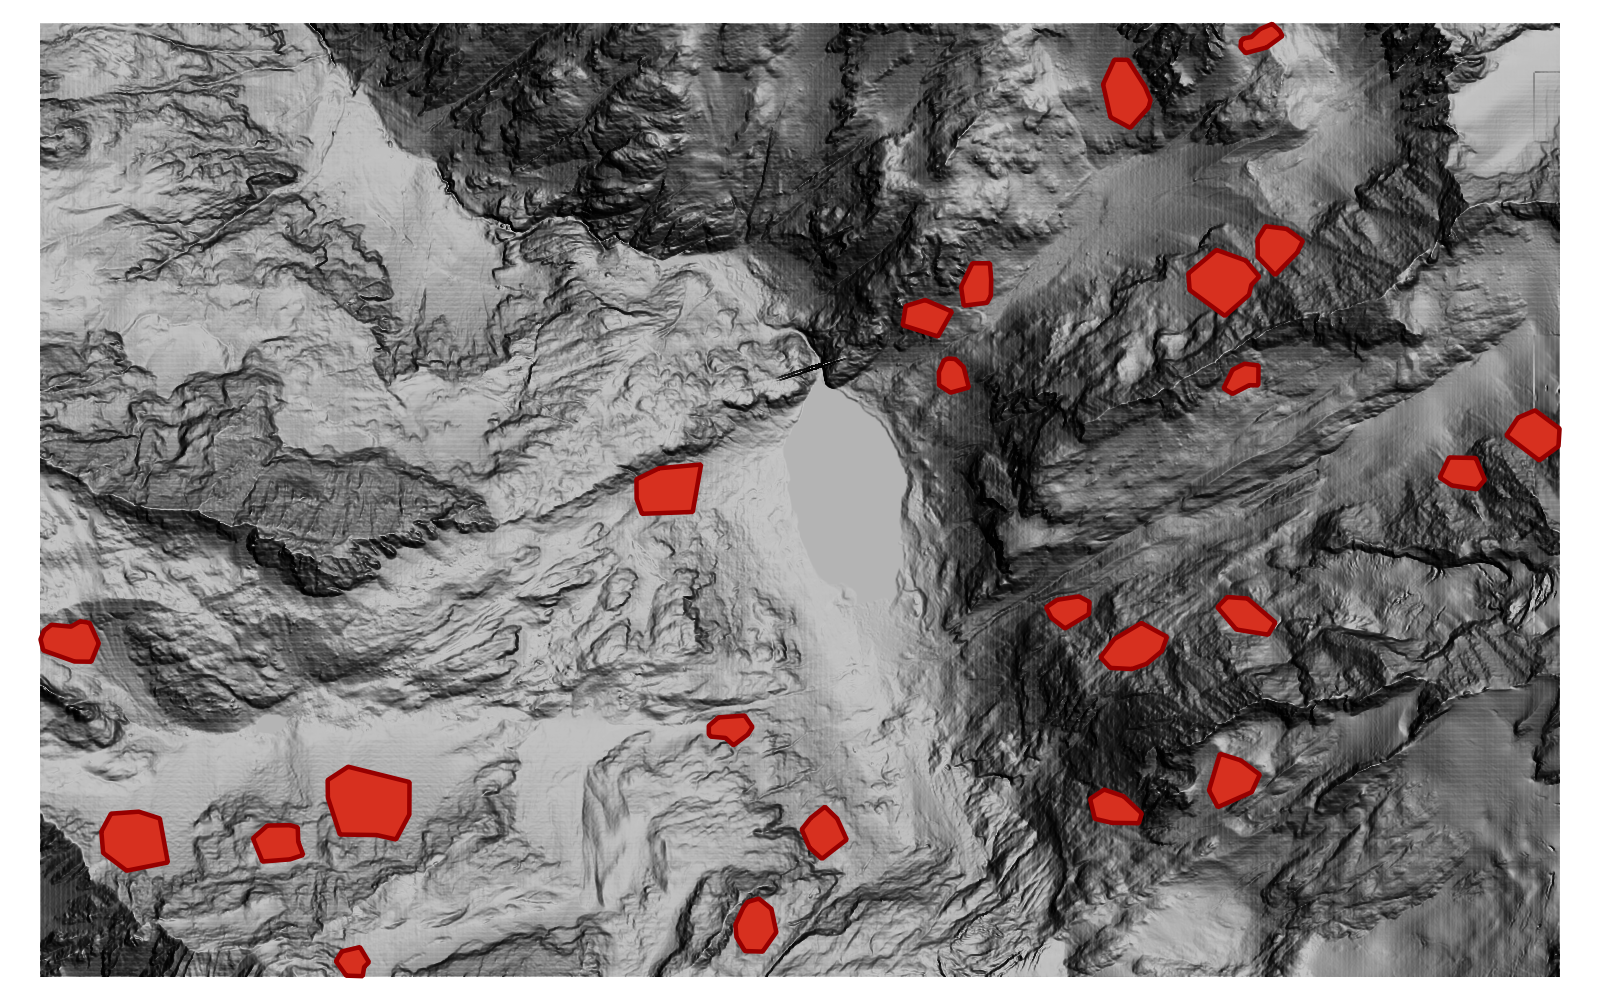
\includegraphics[width=.86\textwidth,height=.48\textheight,keepaspectratio]{images/result_initial_depth_preview.png}
\caption{Preview Initial Depth output for the tutorial release polygons.}
\label{fig:initial-depth-preview}
\end{figure}

\section{Rheology accordion}

Choose the rheological model and enter its physical parameters. The visible
fields describe resistance to motion and, when enabled, how those values vary
with elevation. The interface changes which fields are active according to the
selected model.

Use \control{Visualize Rheology Zones} to create a categorical raster from the
current elevation breaks. Each cell color identifies the zone whose parameters
the solver will apply there. This is a setup check, not a simulation result.

\subsection*{How to enter altitude zones}

Leave \control{Altitude zones} empty to use the single $\mu$, $\xi$, and
cohesion values shown above it everywhere. For altitude-dependent rheology,
enter one comma-separated row per zone in this exact order:

\begin{center}
\pathcode{$\mu$, $\xi$, cohesion (Pa), lower elevation (m)}
\end{center}

The first row is the lowest zone and its fourth field must remain blank. Every
following row begins at the lower elevation written in its fourth field;
those elevations must be strictly increasing. For example:

\begin{center}
\begin{tabular}{@{}llll@{}}
\pathcode{0.30,} & \pathcode{600,} & \pathcode{0,} & \pathcode{} \\
\pathcode{0.225,} & \pathcode{1200,} & \pathcode{0,} & \pathcode{1680}
\end{tabular}
\end{center}

This applies $\mu=0.30$ and $\xi=600$~m/s$^2$ below 1680~m, and
$\mu=0.225$ and $\xi=1200$~m/s$^2$ at and above 1680~m. Cohesion is zero in
both rows. The solver uses $\xi$ for the Voellmy variants and cohesion only
for cohesive Voellmy; the Coulomb model uses $\mu$. All four columns are still
required so that the zone definition has one unambiguous format.

\begin{importantbox}
Check the categorical raster whenever altitude-dependent values are used.
Every usable DEM cell must receive the expected zone, including cells above
the highest breakpoint. Parameter meaning and units are summarized in the
separate User Interface Reference.
\end{importantbox}

\uiscreenshot{tutorial_avac_rheology.png}{Rheology accordion with the model controls and rheology-zone visualization button.}

\resultfigure{result_rheology_zones.png}{Visualize Rheology Zones output for the two-zone example. Blue identifies elevations below 1680~m and green identifies elevations at or above 1680~m; the hillshade remains visible beneath the categorical raster.}

\section{Simulation / numerical accordion}

Set the avalanche duration, solver-grid cell size, CFL controls, dry-depth
tolerance, refinement level, and limiter. The current interface uses an open
outer boundary: material leaving the DEM calculation domain is allowed to
leave and is not reflected into the domain.

\begin{importantbox}
The AVAC solver cell size must equal the DEM pixel size or be a whole-number
multiple of it. Both coordinate spans must contain whole solver cells. A
coarser cell reduces cost but also reduces spatial detail. CFL limits must be
internally consistent, and increasing AMR or core count does not replace the
need for a resolution study.
\end{importantbox}

AVAC outputs are written at the fixed interval used by the packaged workflow.
The number of output frames follows from that interval and the requested
duration.

\uiscreenshot{tutorial_avac_numerical.png}{Simulation / numerical accordion. The screenshot shows every numerical control exposed to the user.}

\section{Check, prepare, and run AVAC}

Open the \control{AVAC Run} tab and work from top to bottom:

\begin{enumerate}
  \item Set \control{CPU cores}. The initial value is the number available on
        the machine; reduce it if other applications need resources.
  \item Select \control{Check Environment}. A packaged-runtime installation
        does not require a system compiler or a separate Clawpack installation.
  \item Select \control{Validate Inputs}. Correct every reported preflight
        failure before continuing.
  \item Optionally rerun \control{Preview Initial Depth} and
        \control{Visualize Rheology Zones}.
  \item Select \control{Prepare AVAC Run}. A new, isolated run folder is
        created and the progress bar reports input preparation.
  \item Select \control{Run}. The solver runs asynchronously; the same progress
        area reports simulation progress. \control{Stop} requests a controlled
        termination if the run must be canceled.
  \item Use \control{Show AVAC Log} when diagnostic details are needed. A
        successful run is automatically listed in Results.
\end{enumerate}

Preparation and execution are separate. If any AVAC input or parameter is
changed after preparation, prepare a new run before pressing Run.

\uiscreenshot{tutorial_avac_run.png}{AVAC Run tab. Environment checks, validation, preparation, execution, progress, and the optional log are grouped here.}

\clearpage
\part{WAVE: optional avalanche--lake coupling}

\section{Prerequisite and coupling concept}

Enable the Lake-Wave Extension only after a completed AVAC run with usable
time-dependent results exists. WAVE reads that run without modifying it and
inherits its rectangular calculation bounds, simulation duration, output
times, and temporal origin.

The lake polygon has two distinct roles:

\begin{itemize}
  \item it defines which WAVE cells are initially part of the water body at
        the selected absolute water-surface elevation; and
  \item it defines the internal shoreline where the entering avalanche is
        converted into water mass and momentum sources.
\end{itemize}

At every AVAC output time, the coupling samples avalanche depth and both
horizontal momentum components along the grid-aligned WAVE shoreline. Only
the flux directed from land into the initially wet lake is admitted. The
integrated inward volume flux and its two momentum components are then added
to the WAVE cells adjacent to that shoreline. Cells outside the initial lake
are not permanently forced dry, so runup can wet terrain beyond the polygon.

\begin{notebox}
The polygon is not the WAVE calculation domain. It separates the initial water
body from surrounding terrain and locates the internal avalanche-to-water
transfer.
\end{notebox}

\section{AVAC Source accordion}

Choose the completed AVAC run whose arrival at the lake will generate the
impulse wave. The selector lists completed runs in the working directory; use
\control{Refresh} after a run finishes. The summary below the selector helps
confirm the intended source, duration, and output availability.

\uiscreenshot{tutorial_wave_source.png}{AVAC Source accordion. WAVE preparation always begins from a completed AVAC run.}

\section{Terrain and Lake Inputs accordion}

\begin{enumerate}
  \item Select the terrain DEM. It must cover the AVAC calculation bounds.
  \item Select an existing \control{Lake / water-body polygon}, or create one
        from a water-surface elevation and a clicked point in the DEM-connected
        basin.
  \item Enter the \control{Water level}. This is an absolute elevation in the
        same vertical datum as the DEM, not a water depth.
  \item Enter the WAVE grid cell size and select \control{Preview Water Level}.
        The preview creates the exact solver-grid initial lake state. If these
        inputs remain unchanged, WAVE preparation reuses the cached preview
        rather than calculating it again.
\end{enumerate}

To create the water body without a preexisting polygon, first select the DEM
and enter the absolute water level. Select \control{Create Lake Polygon from
Map Point}; the cursor is armed for one click. Click a DEM cell inside the
intended basin and below the chosen level. The plugin transforms the click to
the DEM CRS and flood-fills only the north--south/east--west connected DEM
cells at or below that elevation. Other low areas that are not connected to
the clicked basin are excluded. The connected mask is converted to a
GeoPackage in \pathcode{derived\_inputs/}, loaded into QGIS, and selected as
the lake polygon. A right click cancels point capture.

The connected contour must close inside the terrain DEM. If it reaches a DEM
edge, use a DEM that fully encloses the water body or reconsider the water
level. After the polygon is created, select \control{Preview Water Level}.
This resamples the terrain and polygon onto the chosen WAVE grid, sets the
initial water surface to the absolute level, and displays water depth
($h=\max(0,\eta_0-z)$) in the connected lake cells. Inspecting this exact
solver-grid preview catches shoreline differences introduced by a coarser
WAVE cell size before preparation.

\begin{importantbox}
The WAVE DEM must have a valid projected CRS and square pixels. Its cell size
must equal the DEM resolution or be a whole-number multiple of it, and each
inherited AVAC-domain span must contain at least two whole WAVE cells. The lake
polygon and DEM must overlap. A zero water-surface elevation does not mean
``empty lake''; it is interpreted as an absolute elevation in the DEM datum.
\end{importantbox}

\uiscreenshot{tutorial_wave_lake.png}{Terrain and Lake Inputs accordion, including the two lake-polygon paths and exact water-level preview.}

\begin{figure}[htbp]
\centering
\begin{minipage}[t]{.49\textwidth}
\centering
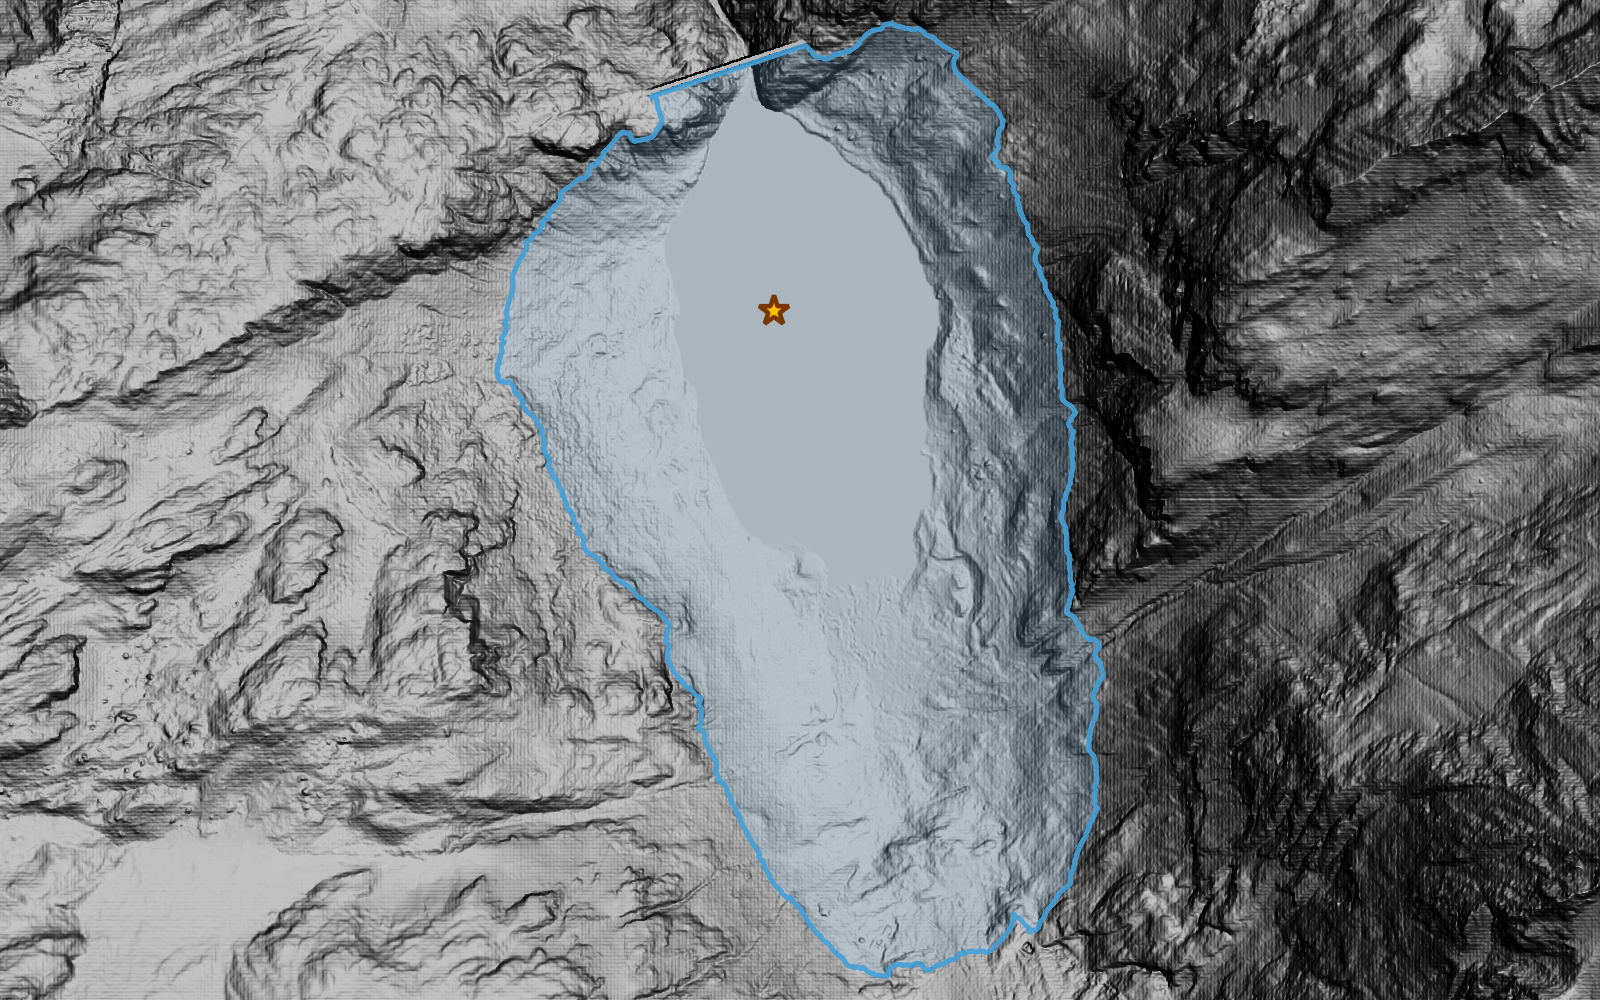
\includegraphics[width=\linewidth]{images/tutorial_lake_polygon_seed.png}
\small (a) Clicked seed (gold star) and the connected water-body polygon.
\end{minipage}\hfill
\begin{minipage}[t]{.49\textwidth}
\centering
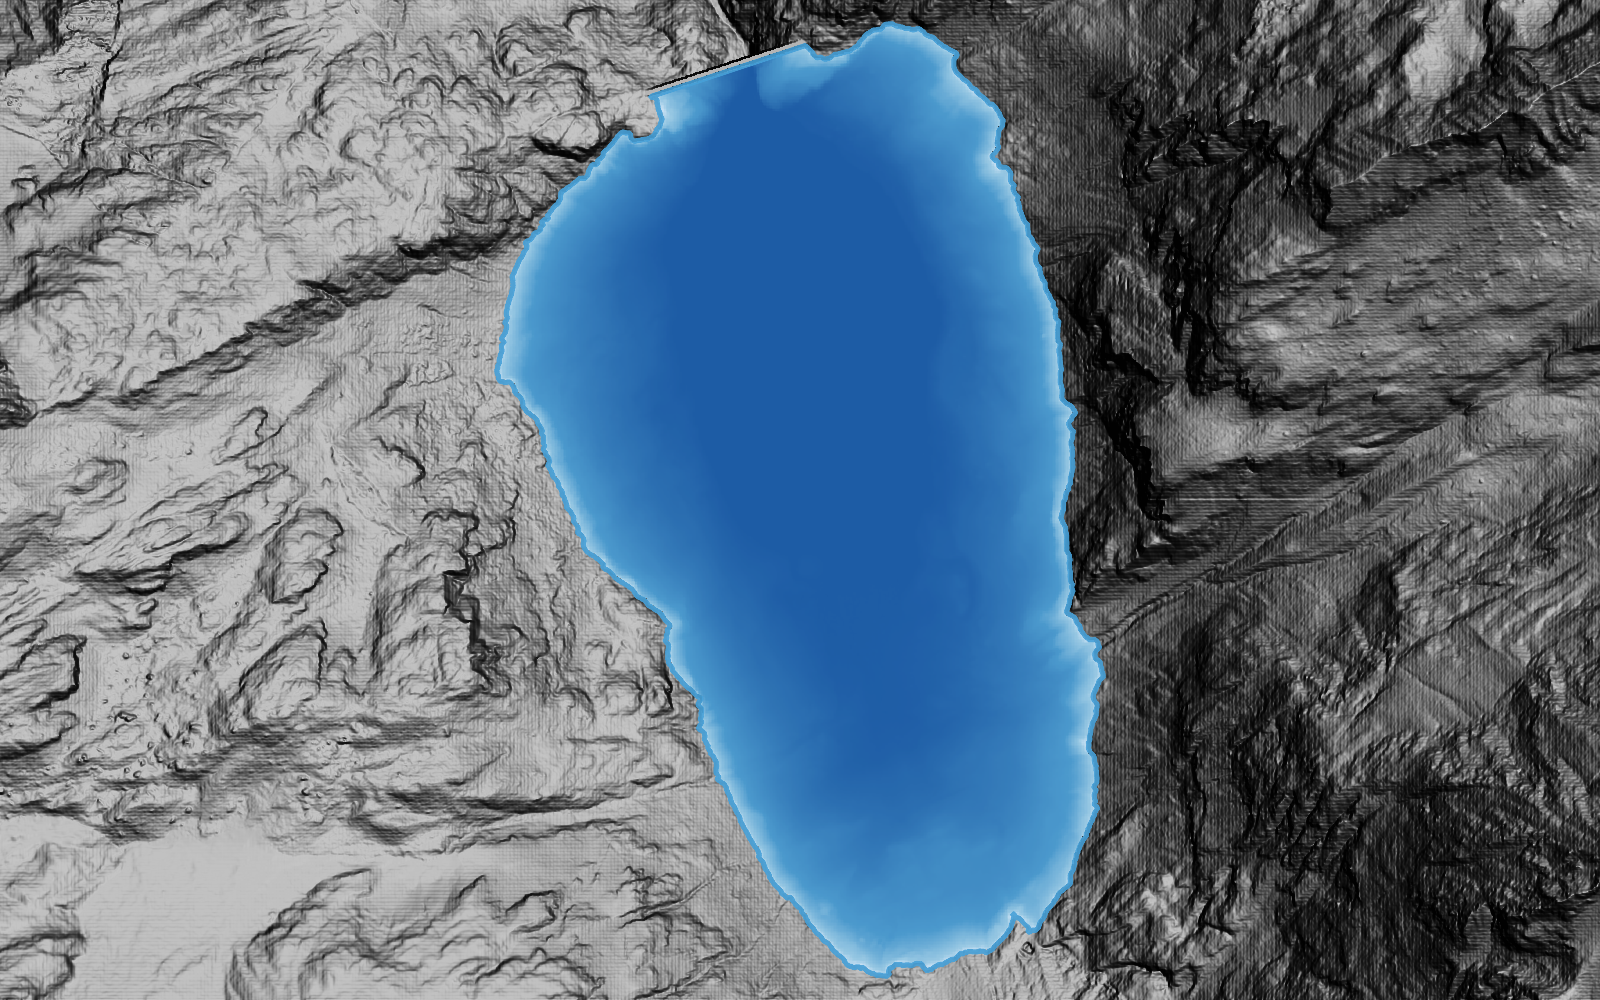
\includegraphics[width=\linewidth]{images/tutorial_water_level_preview.png}
\small (b) Exact WAVE-grid initial water-depth preview.
\end{minipage}
\caption{Building and checking the lake. The light-blue outline is the derived connected water-body polygon.}
\label{fig:lake-creation-preview}
\end{figure}

\section{WAVE Model Settings accordion}

Review the dry-depth threshold, CFL controls, damping and friction settings,
refinement, limiter, and maximum solver steps. These values govern wet/dry
behavior, numerical stability, energy loss, bed resistance, and computational
cost. Use physically justified values and keep the CFL target below its
maximum.

At the bottom of WAVE Parameters, \control{Load WAVE Configuration} and
\control{Save WAVE Configuration} transfer only the WAVE setup. They do not
replace the selected AVAC configuration or the complete plugin case.

\uiscreenshot{tutorial_wave_model.png}{WAVE Model Settings accordion and the WAVE-only configuration controls.}

\section{Check, prepare, and run WAVE}

Open \control{WAVE Run} and follow the same execution pattern as AVAC:

\begin{enumerate}
  \item Set the desired \control{CPU cores} and select
        \control{Check Environment}.
  \item Select \control{Validate Inputs}. WAVE verifies the completed AVAC
        source, terrain, polygon, preview state, inherited domain, and solver
        settings.
  \item Select \control{Prepare WAVE Run}. Preparation builds a new WAVE
        scenario, the initial water state, and the internal shoreline source.
        If no avalanche mass crosses into the lake, preparation stops with a
        clear message because there is no impulse wave to simulate.
  \item Select \control{Run}. Watch the progress bar, use \control{Stop} if
        necessary, and enable \control{Show WAVE Log} only when detailed output
        is useful.
\end{enumerate}

The preparation summary records transferred volume and both horizontal
momentum components. This ledger is the first coupling diagnostic to inspect
when the simulated wave appears too small, too large, or directed incorrectly.

\uiscreenshot{tutorial_wave_run.png}{WAVE Run tab. It mirrors the AVAC check--validate--prepare--run sequence.}

\clearpage
\part{Results: maps, animations, profiles, and histories}

\section{Select completed results}

The final Results tab is shared by AVAC and WAVE. When WAVE is disabled, WAVE
controls are hidden. When it is enabled, AVAC and WAVE result selectors appear
together and all compatible variables use one temporal origin.

In the \control{Results Run} accordion, select a completed AVAC run and, when
needed, its completed WAVE scenario. Use the refresh buttons if a run has just
finished. The summaries identify what is selected; loading a new result does
not alter solver output.

\uiscreenshot{tutorial_results_runs.png}{Results Run accordion with completed AVAC and WAVE sources selected together.}

\section{Summary Maps accordion}

Summary maps collapse the complete simulation into one raster. AVAC provides
peak snow depth, velocity, dynamic pressure, arrival time, and the time of
selected maxima. WAVE provides maximum water-surface rise and maximum
drawdown. Choose a map and select \control{Load Summary Map}.

\uiscreenshot{tutorial_results_summary.png}{Summary Maps accordion. AVAC and WAVE products are selected from the same control.}

\begin{figure}[htbp]
\centering
\begin{minipage}[t]{.49\textwidth}
\centering
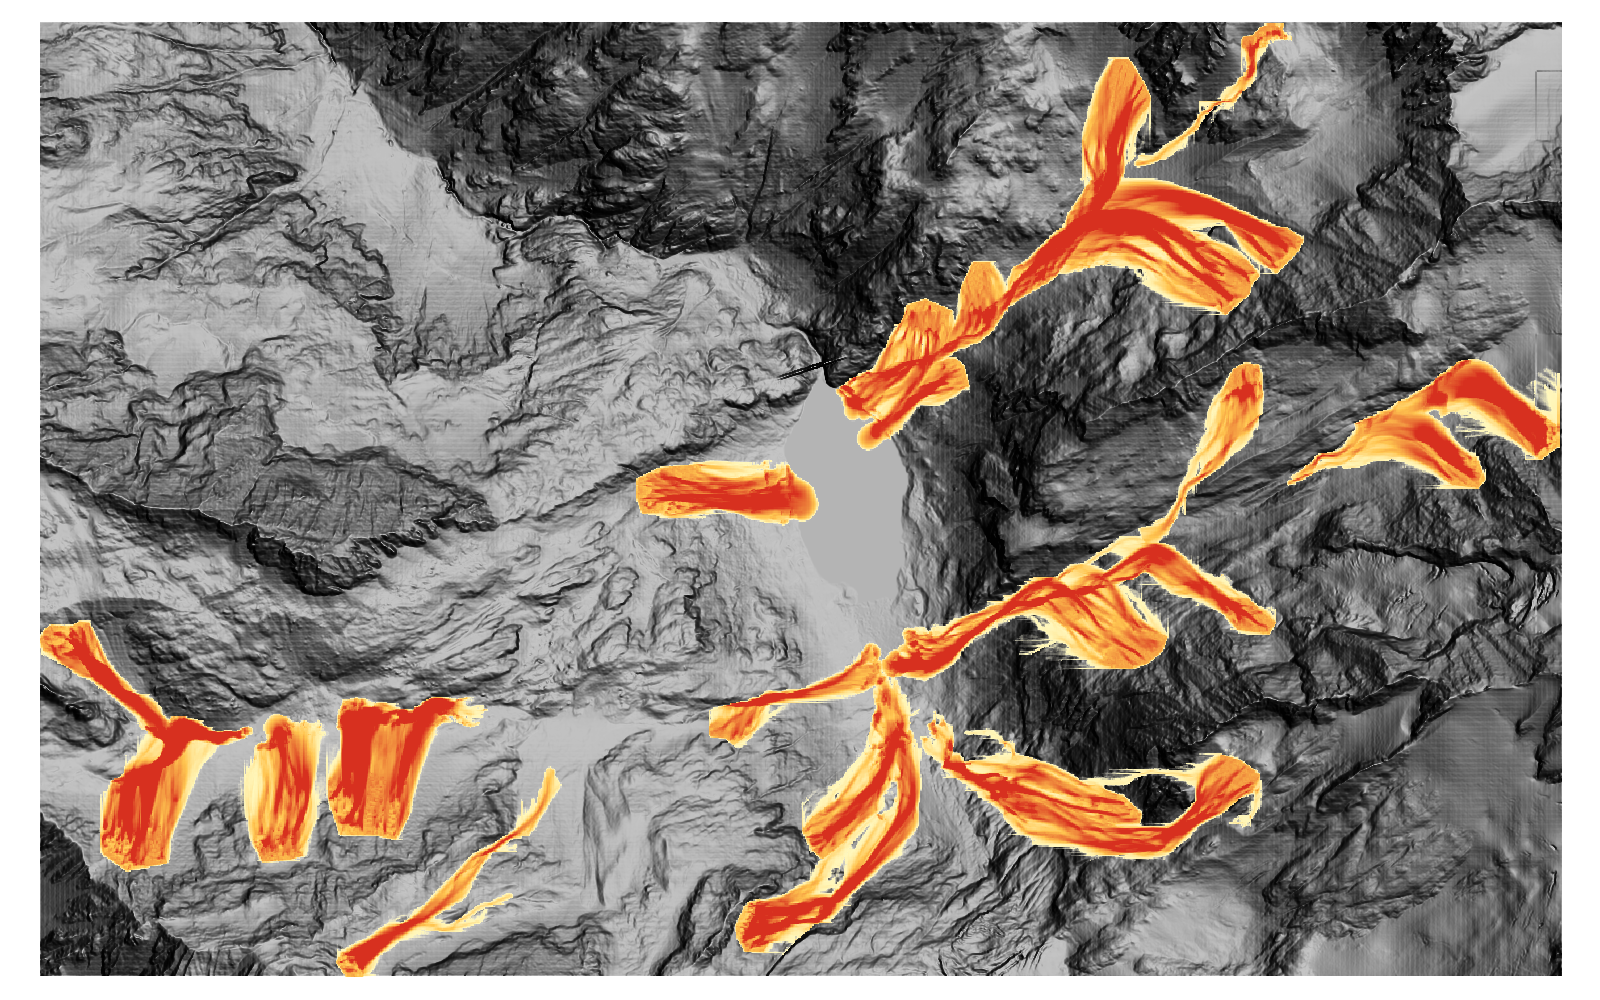
\includegraphics[width=\linewidth]{images/result_summary_avac_max_depth.png}
\small (a) AVAC peak avalanche depth.
\end{minipage}\hfill
\begin{minipage}[t]{.49\textwidth}
\centering
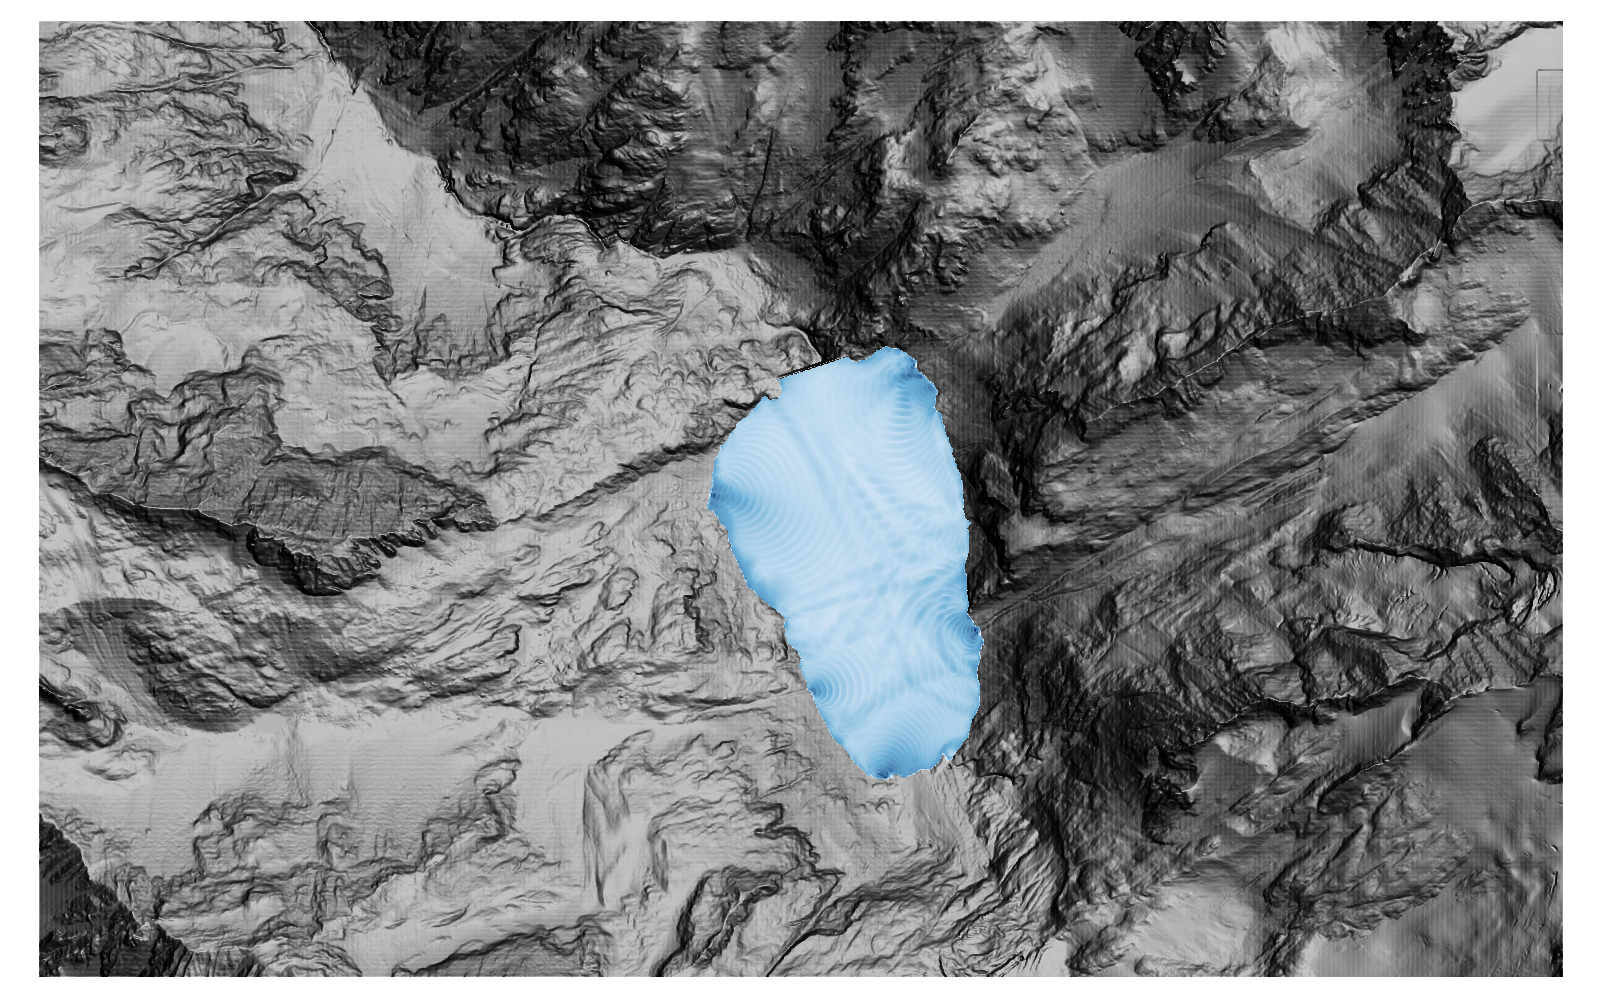
\includegraphics[width=\linewidth]{images/result_summary_wave_rise.png}
\small (b) WAVE maximum surface rise.
\end{minipage}
\caption{Examples of solver-wide summary rasters. Transparent zero values keep the terrain visible.}
\end{figure}

\section{Time Series Maps accordion}

Temporal maps retain one raster band per simulation frame. AVAC variables
include snow depth, velocity, pressure, and snow-surface elevation. WAVE
variables include water depth, water elevation, surface displacement, and the
derived avalanche depth outside the lake. Load a variable, then use the frame
slider, play/pause controls, or the PNG export tools.

The PNG export can write the current frame or the full series, uses the common
simulation timeline, and can include legends and a scale bar. Full-series
exports report progress and can be canceled. A missing temporal layer needed
by another Results tool is loaded automatically.

\begin{importantbox}
For a coupled visualization, use \control{WAVE Snow Depth Outside Lake}
together with \control{WAVE Surface Displacement}. The first is the AVAC depth
with the initial lake-polygon area set to zero; the second shows water rise and
drawdown with zero displacement transparent. The original AVAC result
is not modified.
\end{importantbox}

\uiscreenshot{tutorial_results_temporal.png}{Time Series Maps accordion with playback, layer loading, and PNG export controls.}

\resultfigure{result_temporal_combined.png}{Recommended coupled frame: avalanche depth outside the lake over the diverging water-surface displacement. The semitransparent light-blue polygon and blue border show where the initial lake begins.}

\section{Profile Analysis accordion}

Create or load a QGIS line layer. A convenient method is to create a temporary
scratch line layer in the project CRS, toggle editing, and digitize the desired
cross section over the DEM. Save the layer if it must persist with the case.
The \control{Profile feature} list allows a feature to be chosen directly; a
manual QGIS selection is not required. Then choose the AVAC or WAVE variable
and one of three profile modes:

\begin{itemize}
  \item the currently selected temporal frame;
  \item the complete temporal series, exportable as CSV or PNG frames; or
  \item the historical maximum at every sampled point along the line.
\end{itemize}

Select \control{Extract / Plot Profile} for an interactive plot and
\control{Export Profile CSV} for sampled distance and values. WAVE
water-surface profiles show terrain, water fill, and water elevation; the same
profile style is used consistently for compatible AVAC quantities.

\uiscreenshot{tutorial_results_profile.png}{Profile Analysis accordion. Result source, variable, frame mode, line layer, and feature are chosen in one place.}

\begin{figure}[htbp]
\centering
\begin{minipage}[t]{.49\textwidth}
\centering
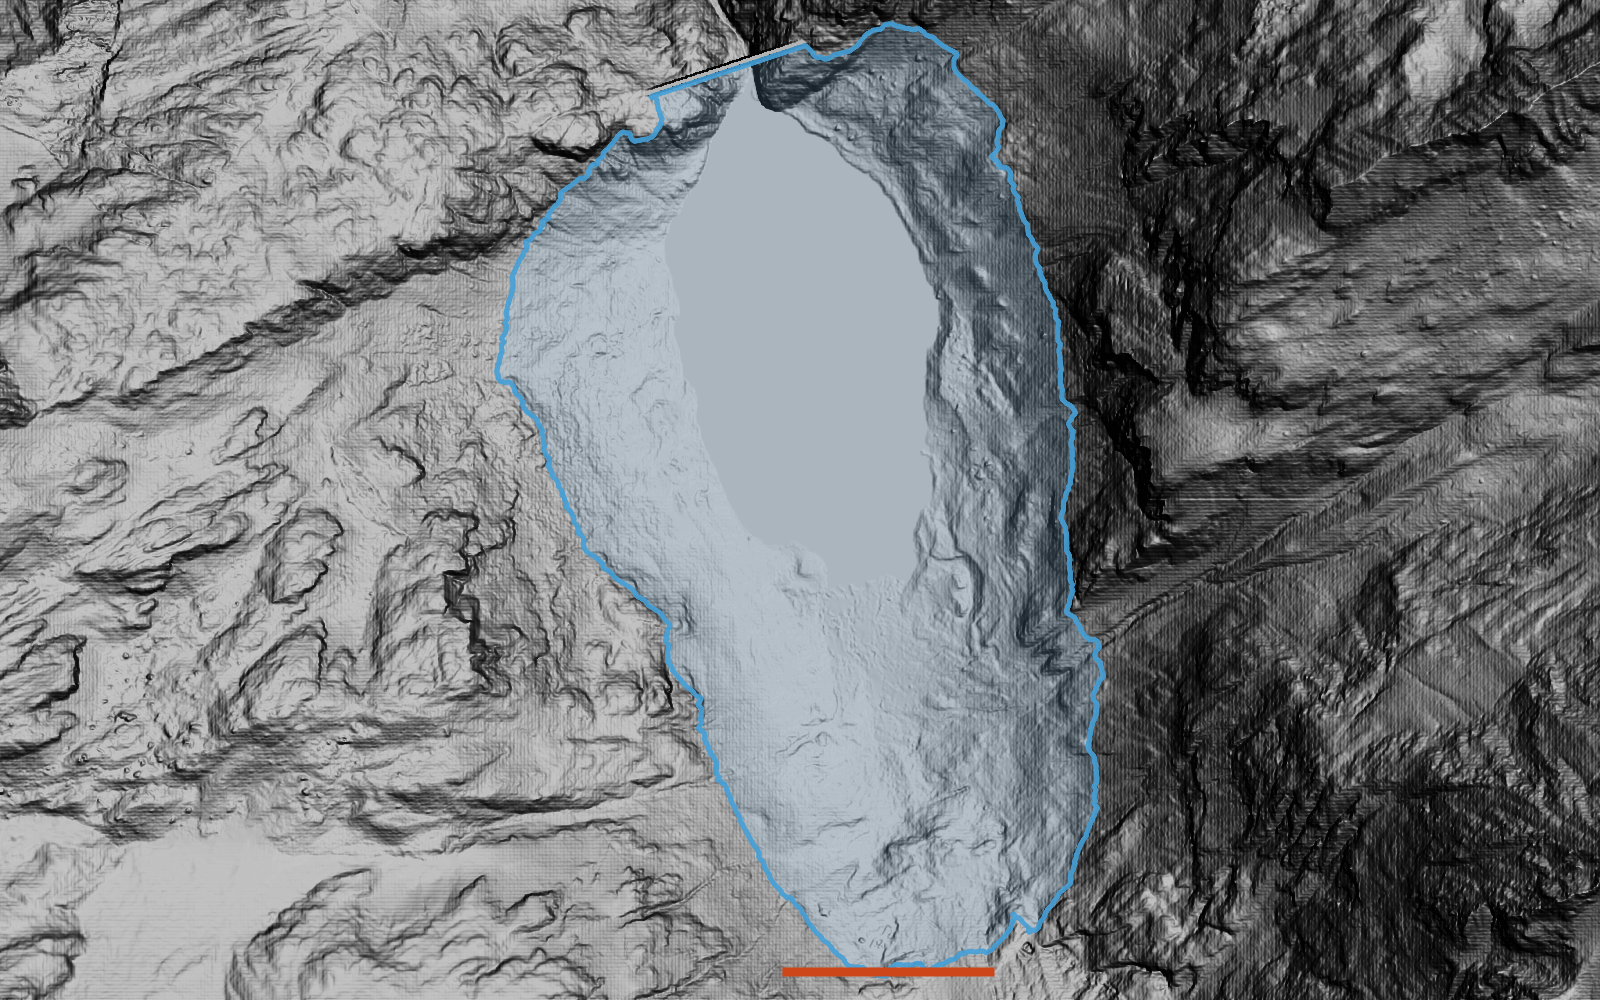
\includegraphics[width=\linewidth]{images/result_profile_location.png}
\small (a) Profile line (orange) digitized over the terrain and lake.
\end{minipage}\hfill
\begin{minipage}[t]{.49\textwidth}
\centering
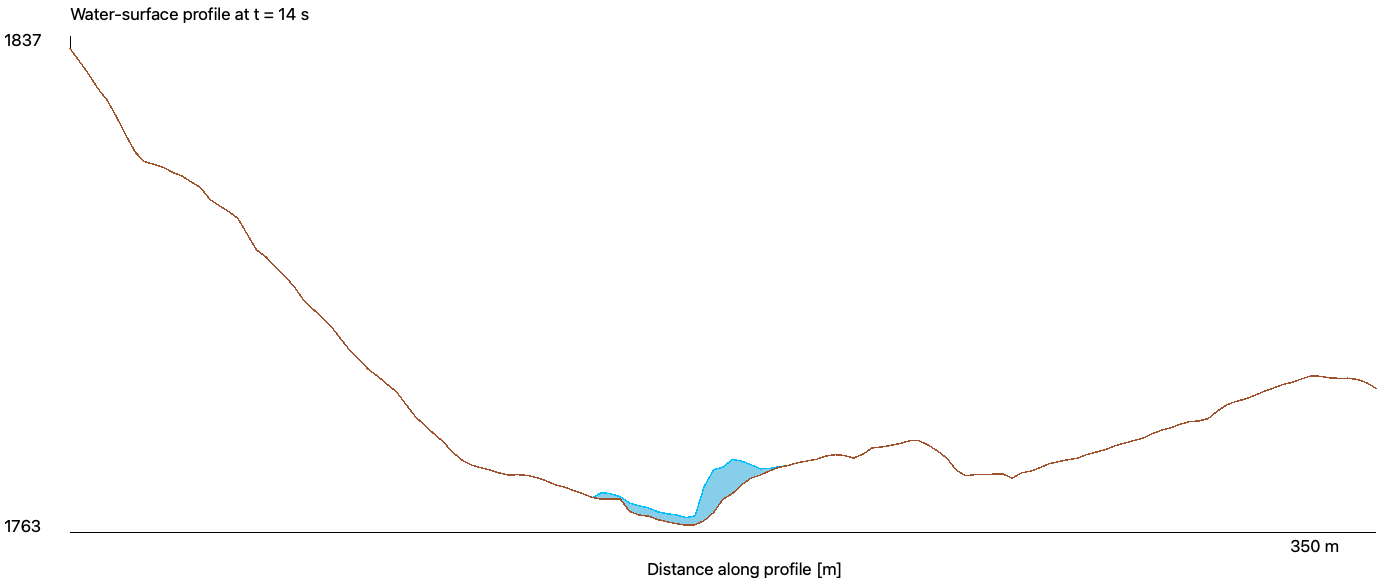
\includegraphics[width=\linewidth]{images/result_profile.png}
\small (b) Extracted terrain and water-surface cross section.
\end{minipage}
\caption{Profile workflow from its QGIS line feature to the resulting plot. The brown line is terrain and the blue fill is the water column.}
\end{figure}

\section{Gauge Histories accordion}

Gauge histories are postprocessing samples. They do not have to be defined
before AVAC or WAVE runs. Load a point layer or create a temporary scratch
point layer in QGIS, toggle editing, and digitize one or more locations over
the DEM. Save the point layer if it must be reused later. Choose an AVAC or
WAVE variable and select \control{Read Gauges from Selected Point Layer}. The
plugin lists the usable point features, transforms their coordinates to the
result CRS, and samples each point through all frames.

Choose a sampled point to plot its history or export simulation time and value
to CSV. If the required temporal product is not loaded, the tool loads it
before sampling.

\uiscreenshot{tutorial_results_gauges.png}{Gauge Histories accordion, shared by avalanche and water variables.}

\begin{figure}[htbp]
\centering
\begin{minipage}[t]{.49\textwidth}
\centering
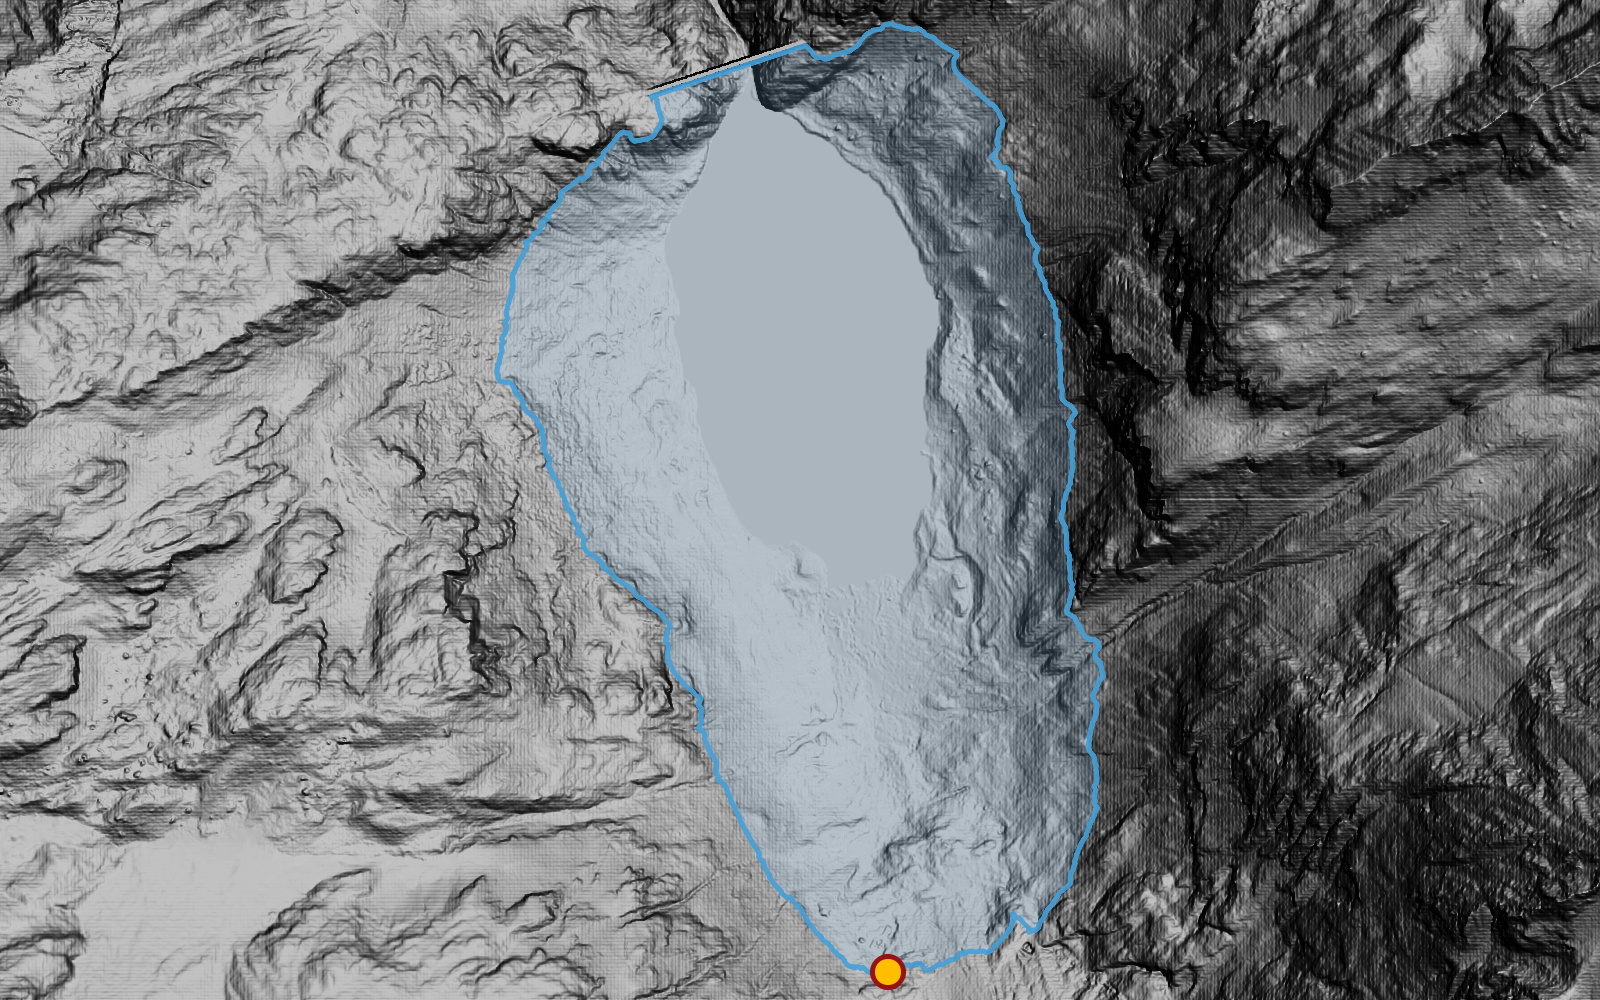
\includegraphics[width=\linewidth]{images/result_gauge_location.png}
\small (a) Gauge point (gold marker) placed on the QGIS map.
\end{minipage}\hfill
\begin{minipage}[t]{.49\textwidth}
\centering
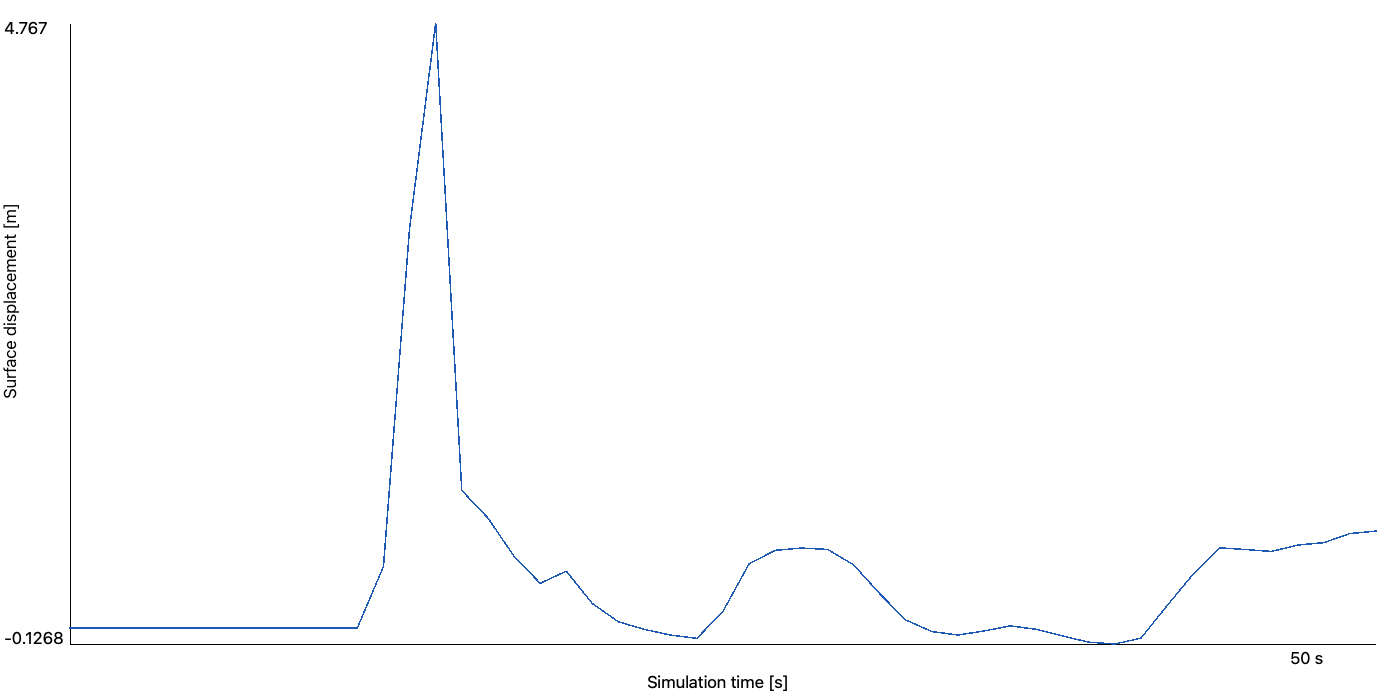
\includegraphics[width=\linewidth]{images/result_gauge_history.png}
\small (b) Sampled water-surface-displacement history.
\end{minipage}
\caption{Gauge workflow from a QGIS point feature to its time-series plot. Later oscillations remain visible after the first arrival.}
\end{figure}

\section{Lake Volume accordion}

This final accordion is visible only when WAVE is enabled. It plots or exports
the lake-water volume at every WAVE output time. Volume is calculated from
water depth and cell area over the initial water-body mask. It is a useful
mass-history diagnostic; the current interface does not provide an outflow or
spillway hydrograph.

\uiscreenshot{tutorial_results_volume.png}{WAVE-only Lake Volume accordion at the end of the Results tab.}

\resultfigure{result_lake_volume.png}{Example lake-water-volume history for a completed coupled simulation.}

\section{Completion checklist}

Before archiving or sharing a case, confirm that:

\begin{itemize}
  \item the complete setup has been saved with \control{Save Case};
  \item the intended AVAC run and, when applicable, WAVE scenario show a
        completed status;
  \item release depth, rheology zones, and initial lake water have been
        visually checked;
  \item the WAVE coupling ledger contains plausible transferred mass and both
        momentum components;
  \item summary maps and the complete temporal sequence have been inspected,
        not only a single attractive frame; and
  \item exported figures and CSV files are stored in the selected AVAC Working
        Directory with enough metadata to identify their run.
\end{itemize}

For a control-by-control description, units, persistence rules, and file
structure, consult the companion \emph{AVAC4QGIS User Interface Guide} in
\pathcode{docs/ui\_reference/}.

\end{document}
